\chapter{Security Analysis}

\section{Formal Security Analysis}

The proposed scheme is translated into ProVerif~\cite{blanchet2018proverif} queries
under the Dolev--Yao adversary model~\cite{dolev1983security}, where the adversary
has full control of the public channel and can intercept, replay, modify, and inject
messages.
All 10 queries are satisfied.
Figure~\ref{fig:proverif} shows the verification output.

\begin{figure}[!ht]
  \centering
  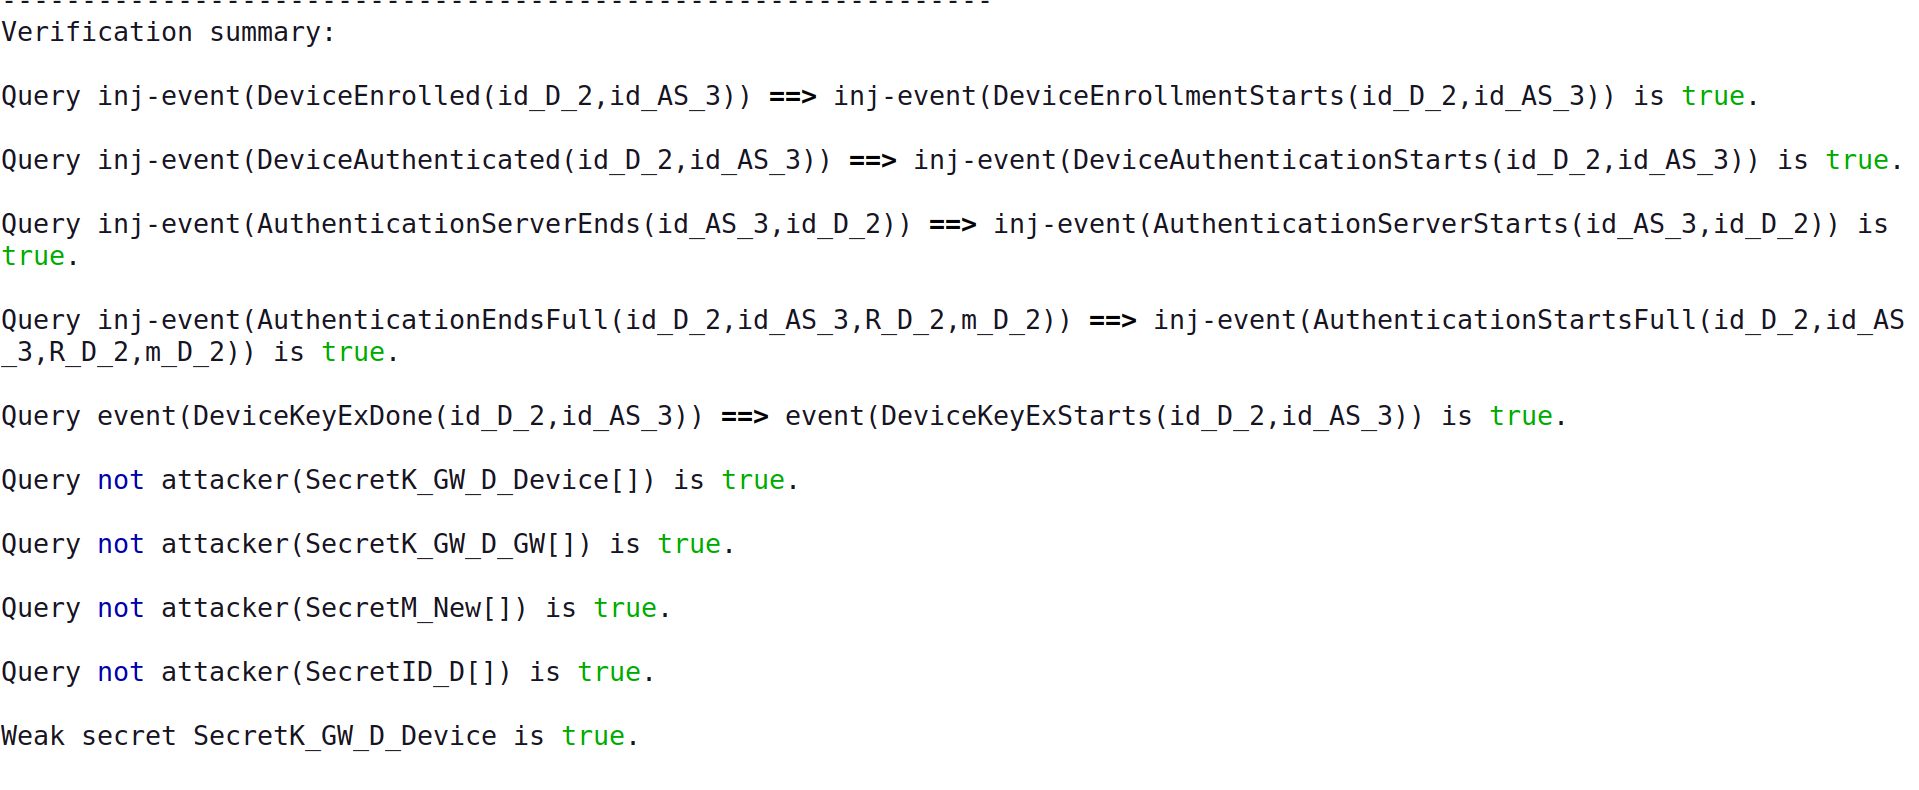
\includegraphics[width=0.98\textwidth]{fig_proverif}
  \caption{ProVerif verification output: all 10 queries satisfied.}
  \label{fig:proverif}
\end{figure}

\subsection{Correspondence Queries (Q1--Q5)}

Five correspondence queries verify that protocol steps occur in the correct order
and that no adversary can skip or forge a step.

\textbf{Q1 (Enrolment correspondence):}
A device can only be enrolled at the authentication server after it has explicitly
initiated the enrolment process.
This ensures a device can only be enrolled with its own participation.

\textbf{Q2 (Authentication, device side):}
The device receives the server's acknowledgement and the fresh timestamp $ts_2$
only after it first sent a valid authentication request.
This prevents replay of a stale acknowledgement.

\textbf{Q3 (Authentication, server side):}
The authentication server completes its processing only after receiving a valid
request from the device.
This rules out an adversary forging a server-side completion event.

\textbf{Q4 (Two-round binding):}
Q4 binds the Authentication and Key Exchange phases: the PUF response $R_D$ and
the session seed $m_{\mathrm{curr}}$ committed during authentication are proven to
be the same values used in the key exchange.
This rules out credential substitution between phases.

\textbf{Q5 (Key exchange correspondence):}
The device recovers the new session seed $m_{\mathrm{new}}$ only after it
legitimately sent the key exchange request.

\subsection{Secrecy and Forward Secrecy (Q6--Q9)}

\textbf{Q6--Q7 (Session key secrecy):}
Two queries verify the secrecy of the session key
$K_{GW\text{-}D} = H(R_D \| m_{\mathrm{new}})$ from the device and gateway
perspectives.
Even though the adversary observes all traffic on the public channel, it cannot
reconstruct $K_{GW\text{-}D}$ because the PUF response $R_D$ is never transmitted
and $m_{\mathrm{new}}$ is always delivered XOR-masked.

\textbf{Q8 (Forward secrecy of $m_{\mathrm{new}}$):}
This query confirms that the rotated session seed $m_{\mathrm{new}}$ remains secret.
Even if an adversary recovers a current session key, it gains nothing about future
sessions because each $m_{\mathrm{new}}$ is derived from an independently generated
fresh nonce.

\textbf{Q9 ($ID_D$ anonymity):}
After enrolment, $ID_D$ is never sent over the open channel again.
Every subsequent message carries the pseudonym
$\mathit{PID} = H(ID_D \| m_{\mathrm{curr}})$.
ProVerif confirms that no attacker, even one who intercepts every message on the
network, can recover $ID_D$ from the observed traffic.

Anonymity is meaningful only if successive pseudonyms are unlinkable.
Since Q8 proves $m_{\mathrm{new}}$ is secret, consecutive pseudonyms
$H(ID_D \| m_{\mathrm{curr}})$ and $H(ID_D \| m_{\mathrm{new}})$ are
computationally indistinguishable to any observer.

\subsection{Offline Guessing Resistance (Q10)}

\textbf{Q10 (Weak secrecy):}
This weak-secrecy query confirms that the session key $K_{GW\text{-}D}$ cannot
be guessed from the public transcript even by an adversary with unlimited offline
dictionary power.
This protects against brute-force and dictionary attacks that try to recover the
key from captured packets.

\section{Informal Analysis}

\subsection{Replay Attack Resistance}

The Enrolment Phase is executed over a secure channel and is immune to replay.
The Authentication and Key Exchange Phases embed timestamps ($ts_1$, $ts_2$,
$ts_{\mathrm{auth}}$) and the session-based random $m_{\mathrm{curr}}$ into the hash
masks.
A replayed message with a stale timestamp or stale $m_{\mathrm{curr}}$ will fail the
freshness check at $AS$, $D$, or $GW$ respectively.

\subsection{MITM Attack Resistance}

The Enrolment Phase is conducted over an encrypted channel, which prevents MITM attacks.
In the Authentication and Key Exchange Phases, the PUF response $R_D$
(device-specific, unreproducible) and session random $m_{\mathrm{curr}}$ (private to
$D$ and $AS$) are embedded in every XOR mask.
Without $R_D$ and the current $m_{\mathrm{curr}}$, no adversary can forge a valid
masked tag $Y_{AS\text{-}D}^H$ or unmask $m_H$.

\subsection{Device Anonymity}

$ID_D$ is transmitted only once, over the secure enrolment channel, and is never
exposed on the open network again.
All open-channel messages use $\mathit{PID} = H(ID_D \| m_{\mathrm{curr}})$,
which is refreshed to $H(ID_D \| m_{\mathrm{new}})$ after every key exchange.
Because $m_{\mathrm{new}}$ is derived from a freshly generated nonce $n_1$,
successive pseudonyms are computationally unlinkable.

\subsection{Desynchronisation Recovery}

Packet loss can occur at three distinct points in the Authentication and Key Exchange
Phases, each handled without requiring re-enrolment.

If the acknowledgement and fresh timestamp $ts_2$ sent by $AS$ to $D$ at the end of
the authentication phase are lost in transit, $D$ does not advance its internal state.
Since $AS$ has not yet performed any state update at this stage, both entities remain
consistent.
Upon timeout, $D$ retransmits the authentication request with the same $\mathit{PID}$
and $ts_1$, and the exchange proceeds normally.

The primary desynchronisation scenario arises when the Key Exchange Phase response
$(m_H, ts_2)$ is lost.
In this case, $AS$ has already advanced its state to $m_{\mathrm{new}}$ and rotated
the pseudonym to $\mathit{PID}_{\mathrm{new}}$, while $D$ retains the previous
$m_{\mathrm{curr}}$.
On the next authentication attempt, $D$ constructs its pseudonym from the stale
$m_{\mathrm{curr}}$, producing $\mathit{PID}_{\mathrm{old}}$.
$AS$ recognises this via the dual-state lookup and resumes from the consistent prior
state.

If the token forwarded from $AS$ to $GW$ is lost, $D$ re-initiates from the
Authentication Phase; the dual-state storage at $AS$ ensures that this
re-authentication succeeds and a fresh token is forwarded to $GW$.

\enlargethispage{3\baselineskip}
\vspace{-6pt}
\subsection{Forward Secrecy}

$K_{GW\text{-}D} = H(R_D \| m_{\mathrm{new}})$.
Compromise of a session key does not reveal previous session keys because
$m_{\mathrm{new}}$ is independently generated from a fresh nonce and $R_D$ is
PUF-derived.
